\documentclass{beamer}
\usepackage[utf8]{inputenc}
\usepackage{graphicx}
\usepackage{xspace} % Needed for macro \xspace
\usepackage{fancyvrb} % Needed for the Verbatim environment

% Remove navigation controls
\usenavigationsymbolstemplate{}

% Slide numbering
\setbeamertemplate{footline}[frame number]

% Convienence macro
\newcommand{\atweb}{\textbf{@Web}\xspace}

% Macro for writing an RDF triple
\newcommand{\triple}[1]{$\langle$\texttt{#1}$\rangle$}

\title{An introduction to Shape Expressions}
\subtitle{
  And how they can be used to implement integrity and classification constraints
  within the \atweb platform
}
\author{
  Leandro Lovisolo \\
  \footnotesize{\href{mailto:leandro.lovisolo@supagro.inra.fr}
                     {leandro.lovisolo@supagro.inra.fr}}
}
\date{October 5, 2015}
\institute{
  INRA SupAgro and INRIA GraphiK \\
  Montpellier, France
}

\begin{document}

\begin{frame}
  \titlepage
\end{frame}

\begin{frame}
  \frametitle{Outline of the presentation}

  \begin{itemize}
    \item Introduction to Shape Expressions
    \item Examples of integrity and classification constraints for the \atweb
      platform written as Shape Expressions
    \item Comparision with equivalent constraints written as SPARQL queries
    \item Survey of the available libraries implementating of Shape Expressions
  \end{itemize}
\end{frame}

\begin{frame}
  \frametitle{Shape Expressions}
  \framesubtitle{Definition}

  \begin{itemize}
    \item It's a validation language for RDF graphs.

    \pause

    \item Allows specifying patterns, or \textit{shapes}, that triples in an
      RDF graph must conform to.

    \pause

    \item Lets one decide whether a RDF graph satisfies all the required shapes.

    \pause

    \item Also possible to deduce which triples conform to which shapes (useful
      for classification.)

    \pause

    \item Roughly comparable to what the Data Definition Language (DDL) does
      for SQL databases, or what XML Schema does for XML documents.
  \end{itemize}
\end{frame}

\begin{frame}
  \frametitle{Motivating example (I)}

  We're going to model an issue tracking system.

  \pause

  \begin{itemize}
    \item An issue:

    \begin{itemize}
      \item is reported by a user,

      \pause

      \item is reported on some date,

      \pause

      \item can be reproduced by an user on some date,

      \pause

      \item is either assigned or unassigned,

      \pause

      \item is related to other issues.
    \end{itemize}

    \pause

    \item A user:

    \begin{itemize}
      \item has one full name, \textbf{OR}

      \pause

      \item has several given names and one family name,

      \pause

      \item can have one mbox.
    \end{itemize}
  \end{itemize}
\end{frame}

\begin{frame}
  \frametitle{Motivating example (II)}

  \begin{center}
    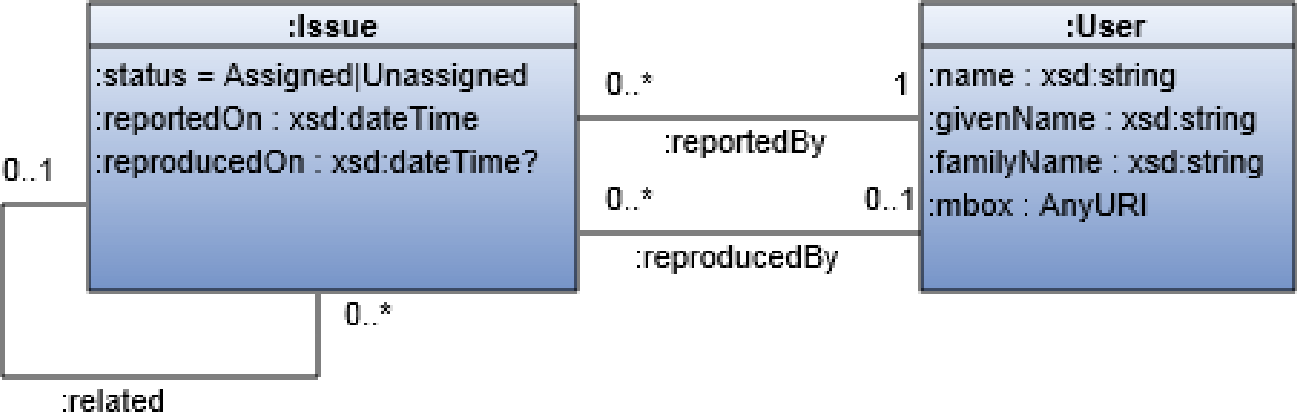
\includegraphics[width=10cm]{schema.png}
  \end{center}
\end{frame}

\begin{frame}[fragile]
  \frametitle{Example data (Turtle syntax)}

  \begin{columns}
    \column{0.5\textwidth}

    \textbf{Valid}

  \begin{Verbatim}[fontsize=\scriptsize]
:Issue1
  :status :unassigned ;
  :reportedBy :Bob ;
  :reportedOn "2013-01-23"^^xsd:date ;
  :reproducedBy :Thompson ;
  :reproducedOn "2013-01-23"^^xsd:date .

:Bob
  foaf:givenName "Bob" ;
  foaf:familyName "Smith" ;
  foaf:mbox <mail:bob@example.org> .

:Thompson
  foaf:givenName "Joe", "Joseph" ;
  foaf:familyName "Thompson" ;
  foaf:mbox <mail:joe@example.org> .
  \end{Verbatim}

    \column{0.5\textwidth}

    \textbf{Invalid}

  \begin{Verbatim}[fontsize=\scriptsize]
:Issue2
  :status :checked ;  # invalid :status.
  :reportedBy :Bob ;
  :reportedOn "2013-01-23"^^xsd:date ;
  :reproducedOn "2013-01-20"^^xsd:date ;
     # missing :reproducedBy.
     # :reproducedOn earlier than
     # :reportedOn.

:Anna
  foaf:givenName "Bob" ;
    # missing :familyName.
  foaf:mbox <mail:bob@example.org> .

:Pete
  foaf:name "Peter", "Pete" ;
    # multiple foaf:names.
  \end{Verbatim}
  \end{columns}
\end{frame}

\begin{frame}[fragile]
  \frametitle{Shape Expression: User}

  \begin{Verbatim}
<UserShape> {
  ( foaf:name xsd:string |
    foaf:givenName xsd:string+ ,
    foaf:familyName xsd:string
  ),
  foaf:mbox shex:IRI ?
}
  \end{Verbatim}
\end{frame}

\begin{frame}[fragile]
  \frametitle{Shape Expression: Issue}

  \begin{Verbatim}
<IssueShape> {
  :status ( :unassigned
            :assigned ),
  :reportedBy @<UserShape>,
  :reportedOn xsd:date,
  ( :reproducedBy @<UserShape>,
    :reproducedOn xsd:date
  )?,
  :related @<IssueShape>*
}
  \end{Verbatim}
\end{frame}

\begin{frame}[fragile]
  \frametitle{The Shape Expressions language (I)}

  \begin{itemize}
    \item Using this language, we define a \textit{schema}.

    \pause

    \item A schema is just a set of \textit{shape expressions}.

    \pause

    \item A shape expression is a labelled \textit{pattern}, e.g.:

    \begin{Verbatim}[fontsize=\scriptsize]
<label>: {
  ... pattern ...
}
    \end{Verbatim}

    \pause

    \item A pattern is a \textit{conjunction} (denoted with a comma) of several
      \textit{expressions}, e.g.:

    \begin{Verbatim}[fontsize=\scriptsize]
<IssueShape>: {
  :status ( :unassigned :assigned ), # an expression
  :reportedBy @<UserShape>,          # another expression
  :reportedOn xsd:date,              # yet another expression
  ...
}
    \end{Verbatim}

  \end{itemize}
\end{frame}

\begin{frame}[fragile]
  \frametitle{The Shape Expressions language (II)}

  An expression can be:

  \begin{itemize}
    \item An \textit{arc rule}, which is a \textit{name
      definition} followed by a \textit{value definition}, e.g.:

    \begin{Verbatim}[fontsize=\scriptsize]
# name definition  # value definition
:reportedOn        xsd:date
    \end{Verbatim}

    \pause

    \item A \textit{group rule} which groups several rules as a single rule
      (useful for cardinality constraints), e.g.:

    \begin{Verbatim}[fontsize=\scriptsize]
( :reproducedBy @<EmployeeShape>,
  :reproducedOn xsd:dateTime )?
    \end{Verbatim}

    \pause

    \item A list of \textit{alternatives} such that the expression matches any
      of the alternatives in the list, e.g.:

    \begin{Verbatim}[fontsize=\scriptsize]
( foaf:name xsd:string |
  foaf:givenName xsd:string+, foaf:familyName xsd:string )
    \end{Verbatim}

  \end{itemize}
\end{frame}

\begin{frame}[fragile]
  \frametitle{The Shape Expressions language (III)}

  The possible \textit{cardinality constraints} are:

  \pause

  \begin{itemize}
    \item \texttt{?} for rules with cardinality 0 or 1, e.g.:

    \begin{Verbatim}
( :reproducedBy @<UserShape>,
  :reproducedOn xsd:dateTime )?
    \end{Verbatim}

    \pause

    \item \texttt{*} for rules with cardinality at least 0, e.g.:

    \begin{Verbatim}
:related @<IssueShape> *
    \end{Verbatim}

    \pause

    \item \texttt{+} for rules with cardinality at least 1, e.g.:

    \begin{Verbatim}
foaf:givenName xsd:string+
    \end{Verbatim}

    \pause

    \item \texttt{$\{m, n\}$} for rules with cardinality between $m$ and $n$.

  \end{itemize}
\end{frame}

\begin{frame}[fragile]
  \frametitle{The Shape Expressions language (IV)}

  A name definition matches predicate names. Can be either:

  \begin{itemize}
    \item an IRI, e.g. \texttt{foaf:name}

    \pause

    \item an IRI prefix, e.g. \texttt{foaf:\~}

    \pause

    \item any predicate except some from a list, e.g.
      ``\texttt{ - foaf:name}'' matches any predicate but \texttt{foaf:name}

    \pause

    \item any predicate at all, denoted by the symbol dot (\texttt{.})
  \end{itemize}
\end{frame}

\begin{frame}[fragile]
  \frametitle{The Shape Expressions language (V)}

  A value definition places a constraint on the kinds of nodes that can
    be referenced by a predicate. Can be either:

  \begin{itemize}
    \item A \textit{value type}, e.g. \texttt{xsd:date}

    \pause

    \item A \textit{value set} matching any nodes within a set, e.g.
      \texttt{(:assigned, :unassigned)}

    \pause

    \item Any value except those in a particular set, e.g.  ``\texttt{ -
      :checked}''

    \pause

    \item A node that has a particular shape, e.g. \texttt{@<UserShape>}
  \end{itemize}
\end{frame}

\begin{frame}[fragile]
  \frametitle{The Shape Expressions language (VI)}

  \textit{Shape inheritance} can be achieved by using the ampersand symbol
  (\texttt{\&}), e.g.:

  \begin{Verbatim}[fontsize=\scriptsize]
<PersonShape> {
    ( foaf:name xsd:string
      | foaf:givenName xsd:string+,
        foaf:familyName xsd:string
    ),
    foaf:mbox IRI
}

<UserShape> {
    & <PersonShape>
}

<EmployeeShape> {
    & <PersonShape>,
    foaf:phone IRI+
}
  \end{Verbatim}
\end{frame}

\begin{frame}[fragile]
  \frametitle{The Shape Expressions language (VII)}

  \textit{Semantic actions} are arbitrary snippets of code that are executed
  after a rule is evaluated.

  \pause

  \begin{itemize}
    \item Possible to express complex validation rules using.

    \pause

    \item Multiple programming languages can be supported, depending on the
      implementation of shape expressions.

    \pause

    \item Other uses: transforming RDF triplets into different formats,
      generating forms for user interfaces automatically, etc.
  \end{itemize}

  \pause

  Example:

  \begin{Verbatim}[fontsize=\scriptsize]
    :reportedOn xsd:dateTime
        %js{ report = _.o; return true; %},
    (:reproducedBy @<EmployeeShape>,
     :reproducedOn xsd:dateTime
        %js{ return _.o.lex > report.lex; %}
        %sparql{ ?s :reportedOn ?rpt . FILTER (?o > ?rpt) %}
    )
  \end{Verbatim}
\end{frame}


\begin{frame}
  \frametitle{An integrity constraint}
  \framesubtitle{Milling solid quantity output relation}

  \begin{center}
  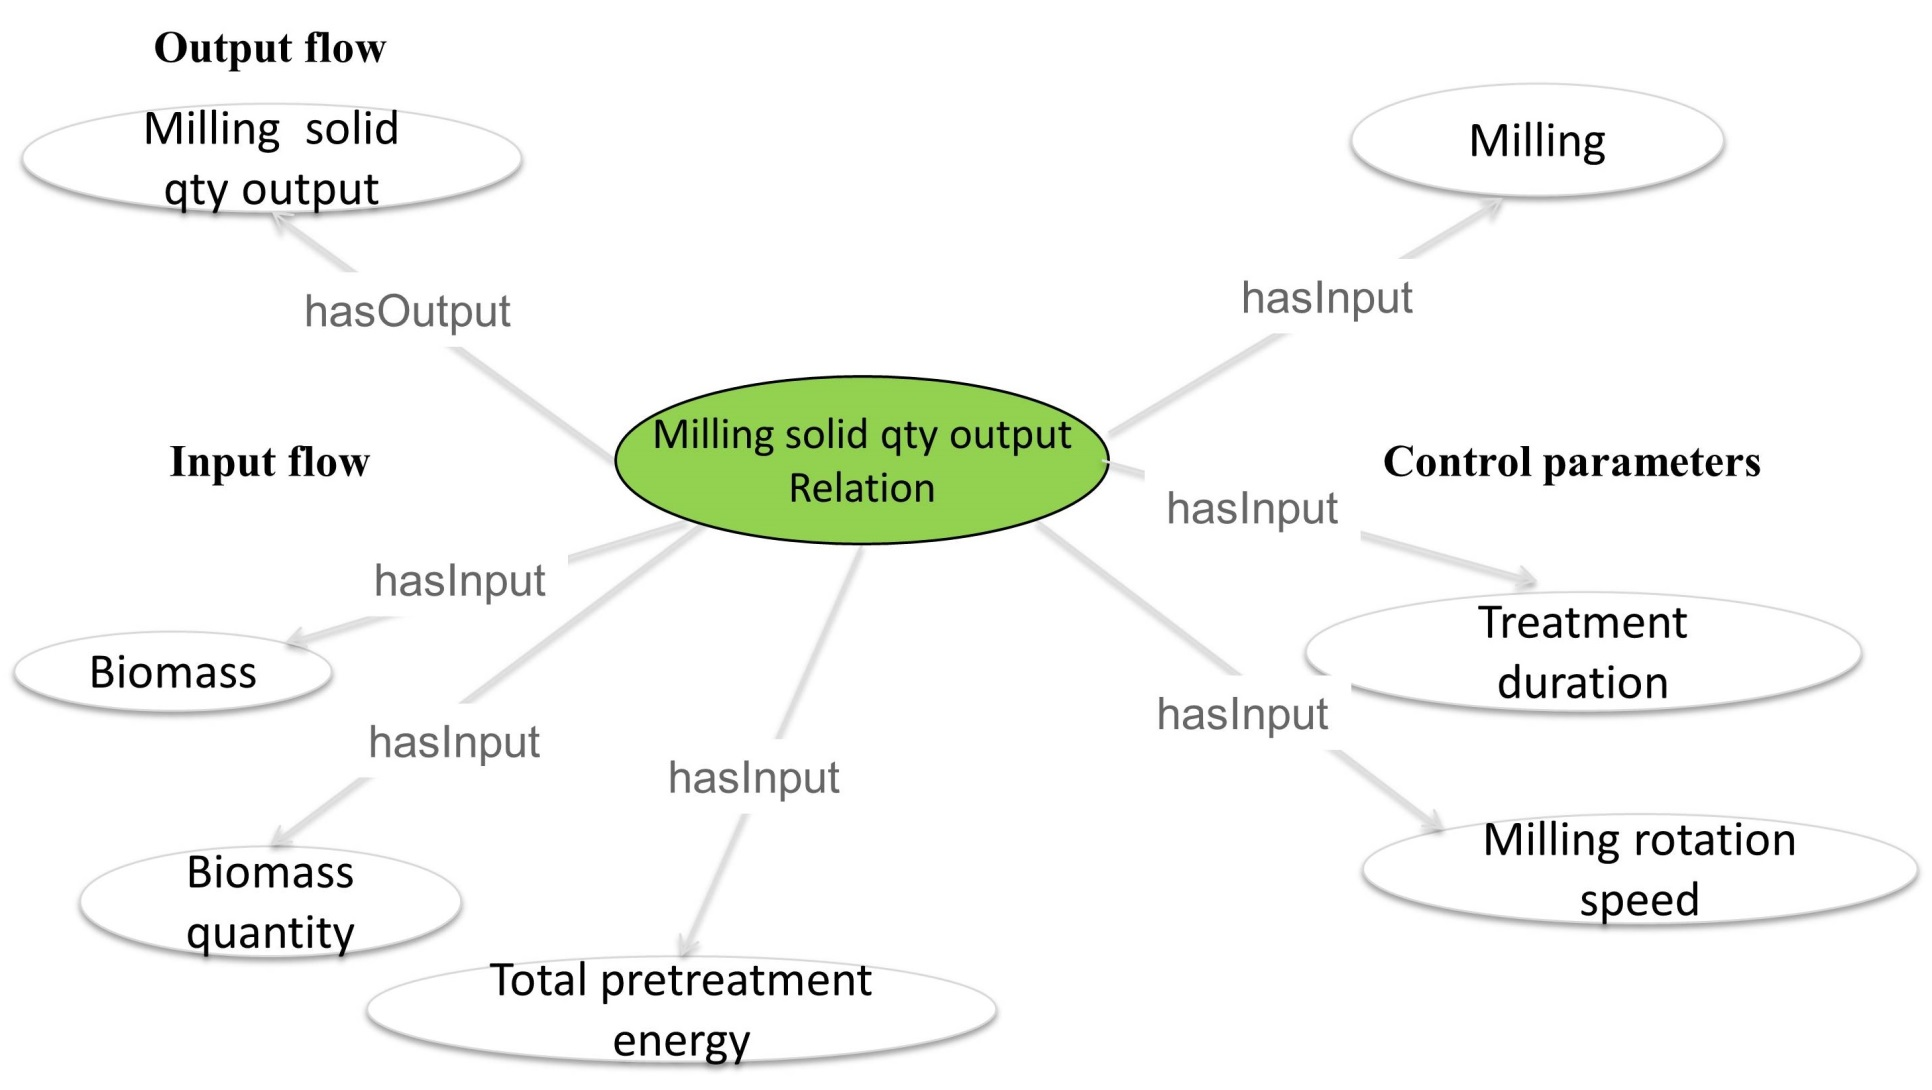
\includegraphics[width=11cm]{relation.jpg}
  \end{center}


\end{frame}

\begin{frame}
  \frametitle{An integrity constraint}
  \framesubtitle{Guideline}

  \textit{``The output quantity of a step is equal to the sum of the quantity
  of water used and the quantity of biomass present in the step.''}
\end{frame}

\begin{frame}[fragile]
  \frametitle{An integrity constraint}
  \framesubtitle{SPARQL query}

  \begin{Verbatim}[fontsize=\tiny]
SELECT ?docid ?doctitle ?tableid ?tabletitle ?rownum  ?solid_qty ?liquid_qty ?output_qty
WHERE {
?doc anno:hasForID ?docid ;
     dc:title ?doctitle ;
     anno:hasTable ?table .

?table anno:hasForID ?tableid ;
       dc:title ?tabletitle ;
       anno:hasForRow ?row .

?row anno:hasForRowNumber ?rownum ;
     anno:hasForRelation [a bioraf:milling_solid_quantity_output_relation ;
                          core:hasAccessConcept ?solid ;
                          core:hasAccessConcept ?liquid ;
                          core:hasResultConcept ?output] .

?solid a bioraf:biomass_quantity ;
       anno:hasForFS [a anno:Scalar ;
                      anno:hasForFuzzyElement /
                      anno:hasForMaxKernel ?solid_qty] .

?liquid a bioraf:water_quantity ;
        anno:hasForFS [a anno:Scalar ;
                       anno:hasForFuzzyElement /
                       anno:hasForMaxKernel ?liquid_qty] .

?output a bioraf:output_solid_constituent_quantity ;
        anno:hasForFS [a anno:Scalar ;
                       anno:hasForFuzzyElement /
                       anno:hasForMaxKernel ?output_qty] .

FILTER (xsd:float(?output_qty) != xsd:float(?solid_qty) + xsd:float(?liquid_qty))
}
  \end{Verbatim}
\end{frame}

\begin{frame}
  \frametitle{An integrity constraint}
  \framesubtitle{Graph view of the SPARQL query}

  \begin{center}
  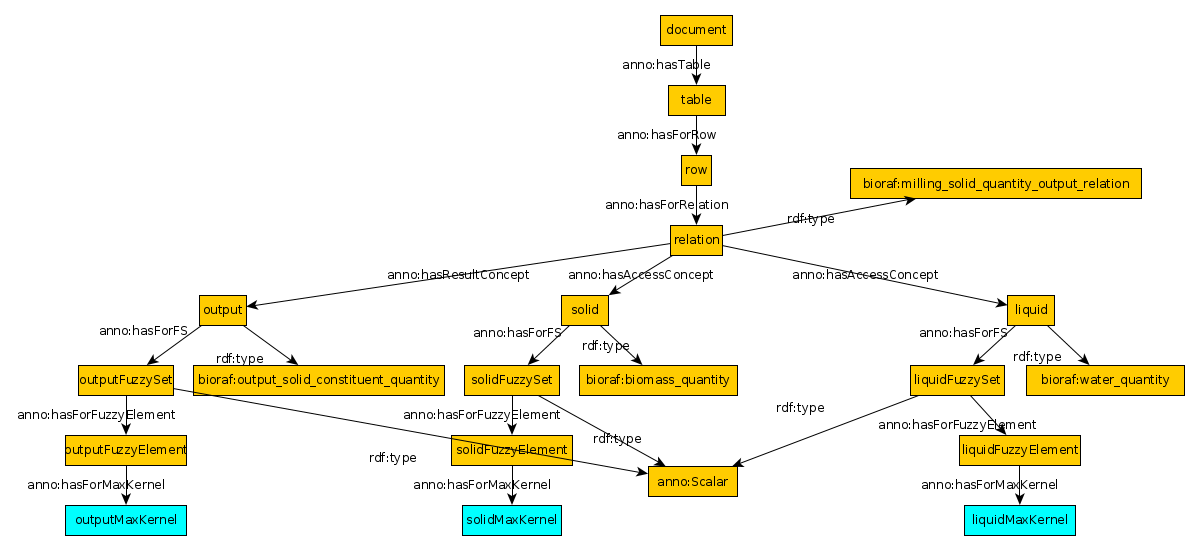
\includegraphics[width=11cm]{integrity-constraint.png}
  \end{center}
\end{frame}

\begin{frame}[fragile]
  \frametitle{An integrity constraint}
  \framesubtitle{Shape Expression}

  \begin{Verbatim}[fontsize=\tiny]
<DocumentShape> { rdf:type anno:Document, anno:hasTable @<TableShape> }
<TableShape> { anno:hasForRow @<RowShape> }
<RowShape> { anno:hasForRelation @<MillingSolidQuantityOutputRelationShape> }

<MillingSolidQuantityOutputRelationShape> {
  core:hasAccessConcept @<SolidAccessConceptShape>,
  core:hasAccessConcept @<LiquidAccessConceptShape>,
  core:hasResultConcept @<OutputResultConceptShape>
}

<SolidAccessConceptShape> {
  rdf:type bioraf:biomass_quantity,
  anno:hasForFS @<FuzzySetShape>
}

<LiquidAccessConceptShape> {
  rdf:type bioraf:water_quantity,
  anno:hasForFS @<FuzzySetShape>
}

<OutputAccessConceptShape> {
  rdf:type bioraf:output_solid_constituent_quantity,
  anno:hasForFS @<FuzzySetShape>
}

<FuzzySetShape> {
  rdf:type anno:Scalar,
  anno:hasForFuzzyElement @<FuzzyElementShape>
}

<FuzzyElementShape> {
  anno:hasForMaxKernel xsd:string
}
  \end{Verbatim}

\end{frame}

\begin{frame}
  \frametitle{A classification constraint}
  \framesubtitle{Guideline}

  \textit{``Topic Bioref-PM: it contains experiments with only one milling
    followed by the enzymatic hydrolysis (Pre-Milling). It does not include a
    physico-chemical step but it can include a washing and separation step. All
    control experiments should be indexed in this topic. (en) ''}
\end{frame}

\begin{frame}[fragile]
  \frametitle{A classification constraint}
  \framesubtitle{SPARQL query}

  \begin{columns}[t]
    \column{0.5\textwidth}
    \begin{Verbatim}[fontsize=\tiny]
SELECT ?docid ?doctitle ?tableid ?tabletitle
       ?rownum1 ?expnum1 ?stepnum1 ?milling
       ?rownum2 ?expnum2 ?stepnum2
WHERE {

VALUES ?milling { bioraf:ball_milling
                  bioraf:wet_disk_milling
                  ... }

?doc anno:hasForID ?docid ;
     dc:title ?doctitle ;
     anno:hasTable [anno:hasForID ?tableid ;
                    dc:title ?tabletitle ;
                    anno:hasForRow ?row1, ?row2] .

?row1 anno:hasForRowNumber ?rownum1 ;
      anno:hasForCell [a bioraf:experience_number ;
                       anno:hasForFS /
                       anno:hasForFuzzyElement /
                       anno:hasForMinKernel ?expnum1] ;
      anno:hasForCell [a bioraf:process_step_number ;
                       anno:hasForFS /
                       anno:hasForFuzzyElement /
                       anno:hasForMinKernel ?stepnum1] ;
      anno:hasForCell /
      anno:hasForFS /
      anno:hasForElement /
      a ?milling .
    \end{Verbatim}

    \column{0.5\textwidth}
    \begin{Verbatim}[fontsize=\tiny]
?row2 anno:hasForRowNumber ?rownum2 ;
      anno:hasForCell [a bioraf:experience_number ;
                       anno:hasForFS /
                       anno:hasForFuzzyElement /
                       anno:hasForMinKernel ?expnum2] ;
      anno:hasForCell [a bioraf:process_step_number ;
                       anno:hasForFS /
                       anno:hasForFuzzyElement /
                       anno:hasForMinKernel ?stepnum2] ;
      anno:hasForCell /
      anno:hasForFS /
      anno:hasForElement /
      a bioraf:enzymatic_hydrolysis_treatment .

FILTER (?expnum1 = ?expnum2 &&
        xsd:float(?stepnum1) < xsd:float(?stepnum2))
}
    \end{Verbatim}
  \end{columns}
\end{frame}

\begin{frame}
  \frametitle{A classification constraint}
  \framesubtitle{Graph view of the SPARQL query}

  \begin{center}
    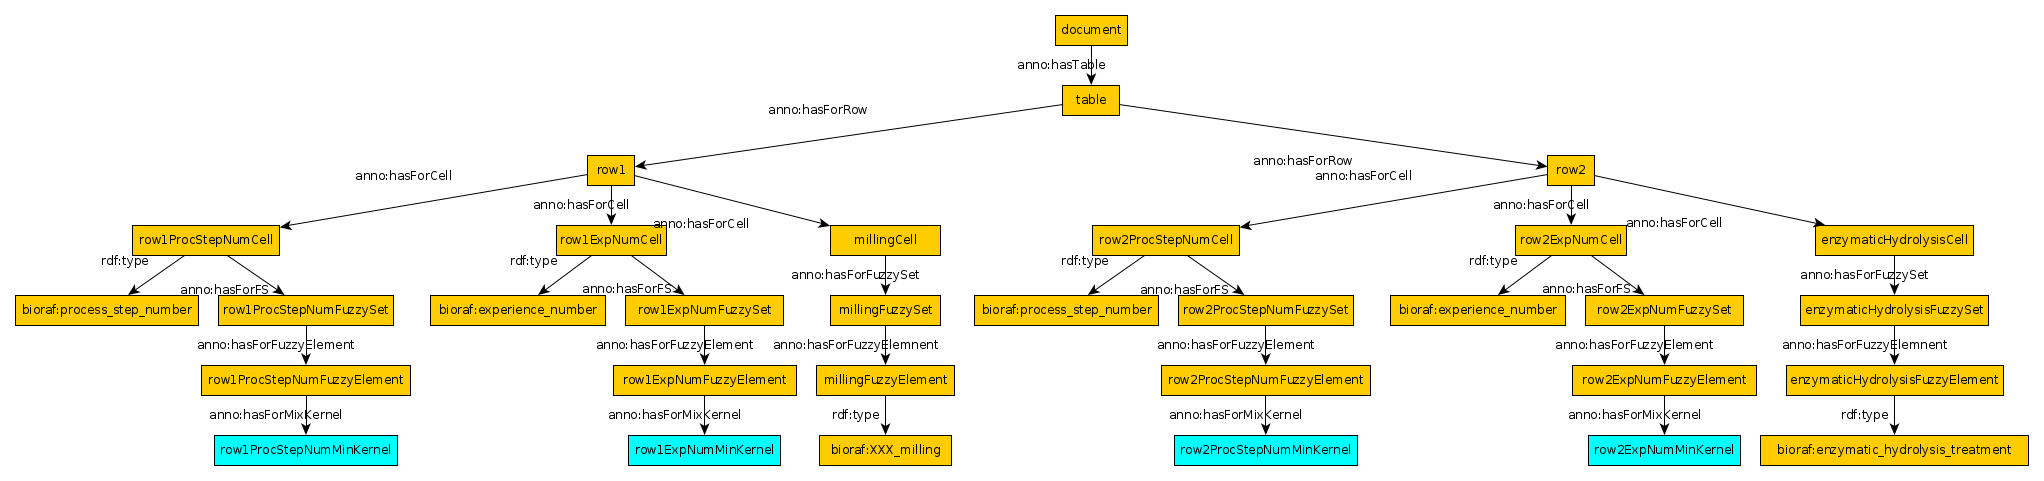
\includegraphics[width=12cm]{classification-constraint.png}
  \end{center}
\end{frame}

\begin{frame}[fragile]
  \frametitle{A classification constraint}
  \framesubtitle{Shape Expression}

  \begin{columns}[t]
    \column{0.5\textwidth}
    \begin{Verbatim}[fontsize=\tiny]
<DocumentShape> {
  rdf:type anno:Document,
  anno:hasTable @<TableShape>
}

<TableShape> {
  anno:hasForRow @<PreMillingRowShape>,
  anno:hasForRow @<EnzymaticHydrolysisRowShape>
}

<PreMillingRowShape> {
  & <RowShape>,
  anno:hasForCell @<PreMillingCellShape>
}

<PreMillingCellShape> {
  & <RowShape>,
  anno:hasForFS @<PreMillingFuzzySet>
}

<PreMillingFuzzySet> {
  anno:hasForElement (bioraf:ball_mlling
                      bioraf:wet_disk_milling ...)
}

<EnzymaticHydrolysisRowShape> {
  anno:hasForCell @<EnzymaticHydrolysisCellShape>
}
    \end{Verbatim}

    \column{0.5\textwidth}
    \begin{Verbatim}[fontsize=\tiny]
<EnzymaticHydrolysisCellShape> {
  anno:hasForFS @<EnzymaticHydrolysisFuzzySet>
}

<EnzymaticHydrolysisFuzzySet> {
  anno:hasForElement bioraf:enzymatic_hydrolysis_treatment
}

<RowShape> {
  anno:hasForRowNumber xsd:integer,
  anno:hasForCell @<ExperienceNumberCellShape>,
  anno:hasForCell @<ProcessStepeNumberCellShape>
}

<ExperienceNumberCellShape> {
  rdf:type bioraf:experience_number,
  anno:hasForFS @<FuzzySetShape>
}

<ProcessStepNumberCellShape> {
  rdf:type bioraf:experience_number,
  anno:hasForFS @<FuzzySetShape>
}

<FuzzySetShape> {
  rdf:type anno:Scalar,
  anno:hasForFuzzyElement @<FuzzyElementShape>
}

<FuzzyElementShape> {anno:hasForMinKernel xsd:string}
    \end{Verbatim}
  \end{columns}
\end{frame}

\begin{frame}
  \frametitle{Libraries implementing Shape Expressions}

  \begin{itemize}
    \item \textit{ShExcala}

    \pause

    \begin{itemize}
      \item Implemented in the Scala programming language

      \pause

      \item Can be used from any JVM language (good for \atweb)

      \pause

      \item \textbf{Doesn't implement semantic actions}
    \end{itemize}

    \pause

    \item \textit{FancyShExDemo}

    \pause

    \begin{itemize}
      \item Implemented in the JavaScript programming language

      \pause

      \item Prototype/proof-of-concept implementation of shape expressions

      \pause

      \item Handles semantic actions

      \pause

      \item Able to generate SPARQL queries
    \end{itemize}
  \end{itemize}
\end{frame}

\begin{frame}
  \frametitle{Statistics for the two SPARQL constraints}

  \pause

  Integrity constraint (milling solid output quantity relation):

  \pause

  \begin{itemize}
    \item Detected \textbf{22} inconsistencies out of \textbf{79} instances of
      the relation.
  \end{itemize}

  \pause

  Classification constraint (BIOREF-PM topic):

  \pause

  \begin{itemize}
    \item Found \textbf{342} candidate experiments in \textbf{30} different
      documents.
  \end{itemize}
\end{frame}

\begin{frame}
  \begin{center}
    \Huge{Thanks!}
  \end{center}
\end{frame}

\end{document}
